\section{Graph coloring}

It's possible to color all countries on any political map (or planar graph) using only 4 colors.
This is example from Wolfram Mathematica's website
(using \href{http://reference.wolfram.com/language/ref/FindInstance.html}{FindInstance}):

\begin{figure}[H]
\centering
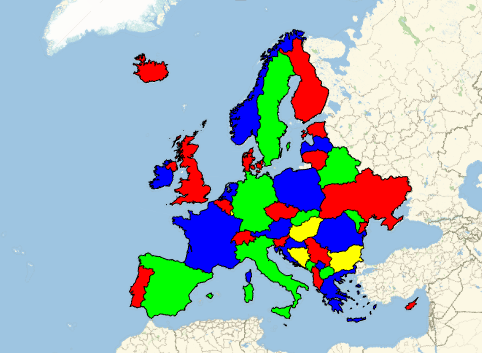
\includegraphics[scale=0.75]{color/map.png}
\caption{Colored map}
\end{figure}

( \url{https://www.wolfram.com/mathematica/new-in-10/entity-based-geocomputation/find-a-four-coloring-of-a-map-of-europe.html} )

Any map or vertices on planar graph can be colored using at most 4 colors.
This is quite interesting story behind this.
This is a first serious proof finished using automated theorem prover (Coq):
\url{https://en.wikipedia.org/wiki/Four_color_theorem}.

An example where I use graph coloring: \ref{tiling_Z3}.

\section{Using graph coloring in scheduling}

I've found this problem in the ``Discrete Structures, Logic and Computability'' book by James L. Hein:

\begin{figure}[H]
\centering
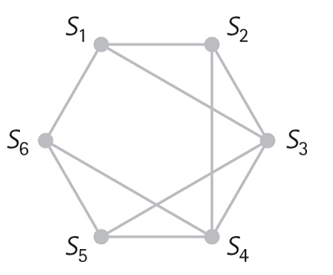
\includegraphics[scale=0.75]{color/fig144.png}
\caption{Graph}
\end{figure}

\begin{framed}
\begin{quotation}
Suppose some people form committees to do various tasks. The problem is to schedule the committee meetings in as few time slots as possible.
To simplify the discussion, we’ll represent each person with a number. For example, let S = {1, 2, 3, 4, 5, 6, 7} represent a set of seven people, and suppose they have formed six three-person committees as follows:

S1 = {1, 2, 3}, S2 = {2, 3, 4}, S3 = {3, 4, 5}, S4 = {4, 5, 6}, S5 = {5, 6, 7}, S6 = {1, 6, 7}.

We can model the problem with the graph pictured in Figure 1.4.4, where the committee names are the vertices and an edge connects two vertices if a person belongs to both committees represented by the vertices.
If each committee meets for one hour, what is the smallest number of hours needed for the committees to do their work?
From the graph, it follows that an edge between two committees means that they have at least one member in common.
Thus, they cannot meet at the same time. No edge between committees means that they can meet at the same time.
For example, committees S1 and S4 can meet the first hour. Then committees S2 and S5 can meet the second hour.
Finally, committees S3 and S6 can meet the third hour. Can you see why three hours is the smallest number of hours that the six committees can meet?
\end{quotation}
\end{framed}

And this is solution:

\lstinputlisting[style=custompy]{color/sched1.py}

The result:

\begin{lstlisting}
hour: 0 committees: [1, 4]
hour: 1 committees: [2, 5]
hour: 2 committees: [3, 6]
\end{lstlisting}

If you increase total number of hours to 4, the result is somewhat sparser:

\begin{lstlisting}
hour: 0 committees: [3]
hour: 1 committees: [1, 4]
hour: 2 committees: [2, 5]
hour: 3 committees: [6]
\end{lstlisting}


\section{Another example}

What if we want to divide our community/company/university by groups.
There are 16 persons and, which must be divided by 4 groups, 4 persons in each.
However, several persons hate each other, maybe, for personal reasons.
Can we group all them so the "haters" would be separated?

\lstinputlisting[style=custompy]{color/sched2.py}

The result:

\begin{lstlisting}
group 0, persons: [1, 2, 5, 8]
group 1, persons: [4, 7, 9, 12]
group 2, persons: [0, 3, 11, 13]
group 3, persons: [6, 10, 14, 15]
\end{lstlisting}



